\subsection{Hardware}
Correspondiente a las pruebas de hardware, se unieron los tres submódulos mencionados anteriormente, el submódulo de sensor, microcontrolador y comunicación inalámbrica. Tras unir cada uno de estos submódulos el resultado es mostrado en la aplicación móvil, dicho resultado es la cantidad de combustible cargado al vehículo.\\
El proceso que se sigue para obtener la cantidad de combustible cargada es el siguiente:
\begin{enumerate}
	\item El flujo de gasolina pasa a través del sensor y este envía una señal cuadrada al microcontrolador.
	\item El microcontrolador recibe la cantidad de flancos de subida que pasan en un segundo por medio del puerto de interrupciones de este mismo.
	\item La cantidad de flancos de subida son transmitidos por medio de los puertos TX y RX al módulo bluetooth para que estos sean enviados al dispositivo móvil.
	\item Los datos son recibidos en la aplicación móvil y se calcula la cantidad de combustible que es recibido en cada segundo.
	\item Tras pasar 10 segundos sin recibir carga de combustible la aplicación móvil muestra la cantidad total cargada al automóvil.
\end{enumerate}
Se realizaron pruebas de todo el proceso descrito anteriormente, los resultados obtenidos se pueden observar en la tabla \ref{pruebas_integracion_combustible}.
\begin{table}[H]
	\centering
	\begin{tabular}{|M{2cm}|M{3cm}|M{3cm}|M{3cm}|M{2cm}|}
		\hline
		\textbf{No. de prueba} & \textbf{Litros esperados} & \textbf{Litros medidos} & \textbf{Error obtenido(litros)} & \textbf{Prueba exitosa}  \\ \hline
		1 & 5  & 5.09 & -0.09 & Si \\ \hline
		2 & 6  & 5.75 & 0.25 & Si \\ \hline
		3 & 8  & 7.65 & 0.35 & Si \\ \hline
		4 & 10  & 9.6 & 0.4 & Si \\ \hline
		5 & 12 &  11.5 & 0.5 & Si \\ \hline
		6 & 14  & 13.4 & 0.6 & Si \\ \hline
		7 & 16  & 15.6 & 0.4 & Si \\ \hline
		8 & 18  & 17.4 & 0.6 & Si \\ \hline
	\end{tabular}
	\caption{Resultados de las pruebas}
	\label{pruebas_integracion_combustible}
\end{table}
La pantalla en la cual se muestran los resultados de todo el procedimiento se puede observar en la figura \ref{fig:prueba_integracion}.
\begin{figure}[H]
	\centering
	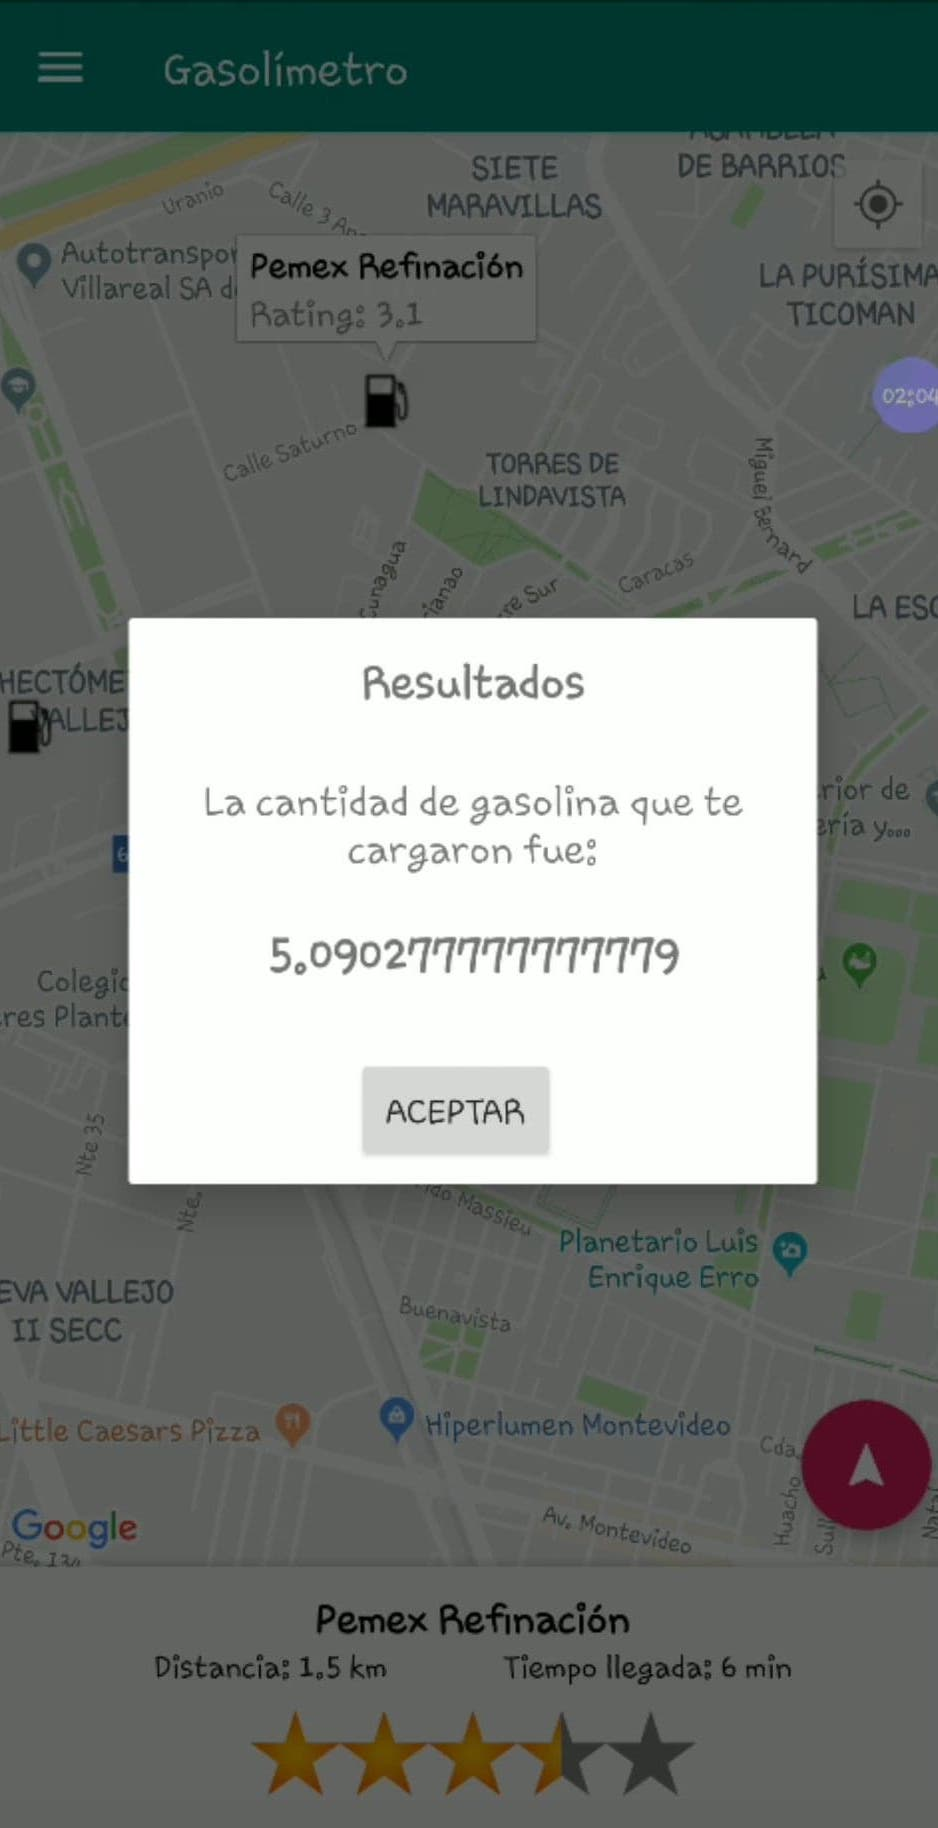
\includegraphics[width=0.5\textwidth]{Capitulo6/integracion/Hardware/img/pantalla_combustible}
	\caption{Resultado de la prueba número uno}
	\label{fig:prueba_integracion}
\end{figure}
